146. \begin{figure}[ht!]
\center{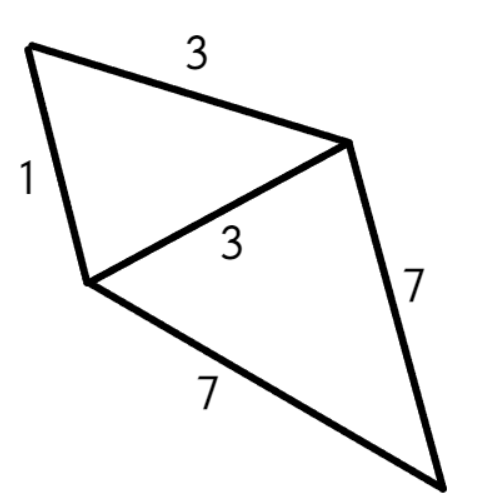
\includegraphics[scale=0.35]{g7-146.png}}
\end{figure}\\
Определим стороны, которые могут быть в равнобедренном треугольнике со стороной 1. Стороны 1, 3 и 7 быть не могут, так как среди них нет равных. Стороны 1, 1 и 3 быть не могут, так как тогда не выполняется неравенство треугольника,  $1+1<3.$ Значит, его стороны могут быть равны только 1, 3 и 3. В другом равнобедренном треугольнике со сторонами 3 и 7 третья сторона может быть равна только 7, так как $3+3<7.$ Значит, периметр исходного четырёхугольника может быть равен только $1+3+7+7=18.$\\
